\begin{figure*}[p]
\centering
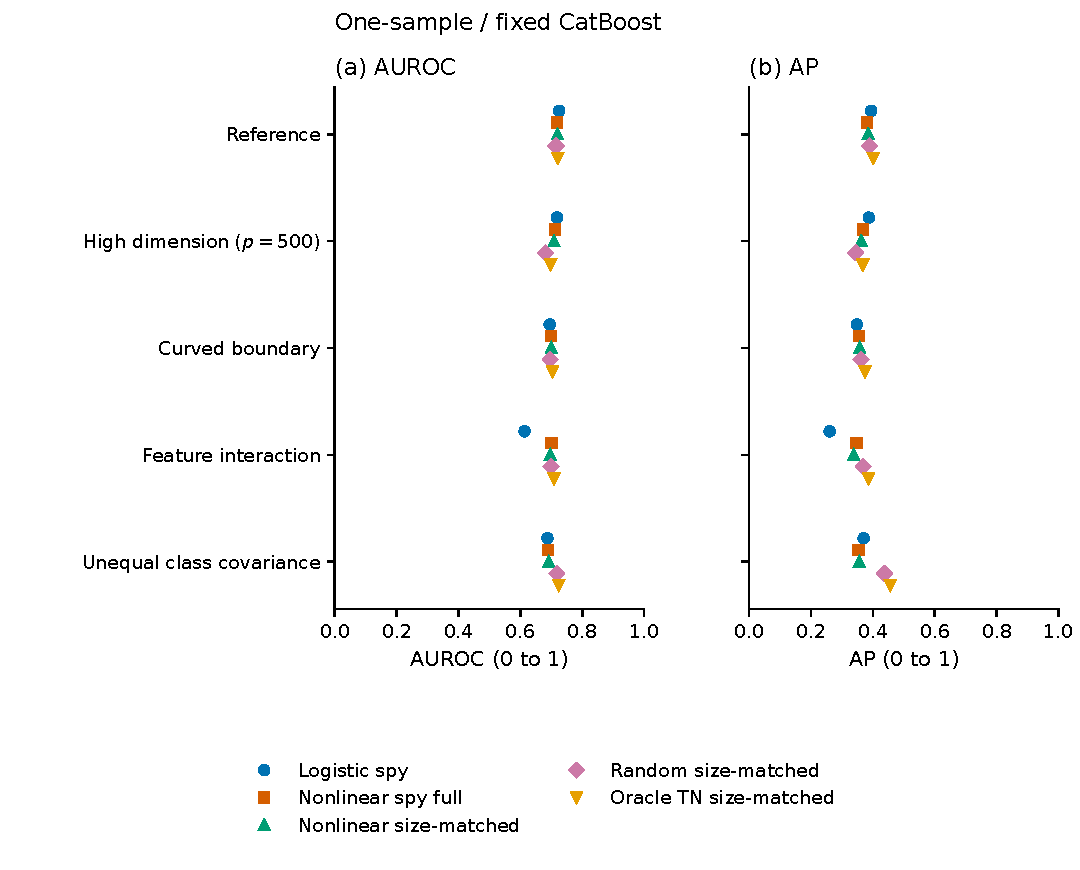
\includegraphics[page=1,width=\textwidth]{revised_figures/fig_s_rn_selector_sensitivity.pdf}
\caption{Diagnostic fixed-parameter CatBoost analysis in five prespecified scenarios. Original logistic spy, full CatBoost nonlinear spy, size-matched nonlinear spy, random size-matched and oracle true-negative size-matched controls are compared. Random/oracle draws are first averaged within each repetition; repetitions are then equally weighted (100 per setting/design). Oracle controls use hidden truth and are not practical PU methods. Nonlinear-spy RN is not added to the benchmark catalog. Plotted absolute AUROC/AP scales are 0 to 1. One-sample / five selection diagnostics. }
\label{fig:s-rn-selector-sensitivity-1}
\end{figure*}
\begin{figure*}[p]
\centering
\includegraphics[page=2,width=\textwidth]{revised_figures/fig_s_rn_selector_sensitivity.pdf}
\caption{Diagnostic fixed-parameter CatBoost analysis in five prespecified scenarios. Original logistic spy, full CatBoost nonlinear spy, size-matched nonlinear spy, random size-matched and oracle true-negative size-matched controls are compared. Random/oracle draws are first averaged within each repetition; repetitions are then equally weighted (100 per setting/design). Oracle controls use hidden truth and are not practical PU methods. Nonlinear-spy RN is not added to the benchmark catalog. Plotted absolute AUROC/AP scales are 0 to 1. Two-sample / five selection diagnostics. }
\label{fig:s-rn-selector-sensitivity-2}
\end{figure*}
